% !TeX spellcheck = de
% HOCHSCHULE REUTLINGEN
% TEMPLATE
% PROF. NOTHOLT

\documentclass[a4paper, 10pt]{IEEEtran}

%%% You can add the packages you may need
\usepackage[bookmarksopenlevel=1, colorlinks=true, allcolors=black, unicode]{hyperref}
\usepackage[cmyk, hyperref, table]{xcolor}
\usepackage{graphicx}


	\title{Regelung eines Dämpfersystems für einen LKW}% Der Titel
	\author{Dustin Walker (763190)% Name und (Matrikel-Nr.)
			-- School of Engineering, Mechatronics Bachelor % Studiengang
			\thanks{Diese Hausarbeit wird in die eingereichte Fassung als Grundlage für die Benurteilung 
		            der Prüfungsleistung für die Prüfung
	            	60040099 % Prüfungsnummer
	            	Regelungstechnik 2. %Prüfungsname
            	 	Der/Die Autor/Autorin versichert, dass dies sein/ihr eigenen Werk ist und alle entnommene Teile anderer Werke richtig zitiert sind.
             		}}
	\markboth
		{Regelungstechnik 2}% Bitte hier das Fach einfügen (Subject)
		{Prüfungsnummer 60040231}% Bitte hier deine Prüfungsnummer einfügen (aus dem HIP)


\begin{document}
	
	\maketitle
	
		
	\begin{abstract} %Hier kommt eine Zusammenfassung des Projektes
		Es soll der Ladebereich eines LKWs aktiv gedämpft werden. Um das System simulieren zu können wird das System in Simulink nachgebaut. Anhand dieses Models soll nun 
		ein Regler entworfen und parametrisiert werden. Es soll ein digitaler Regler benutzt werden. 
		Hierfür muss noch zusätzlich ein Anti Aliasing Filter designt werden.
	\end{abstract}
	
	\section{Einleitung}
	Wenn der Laderaum eines Lkws voll geladen ist und über eine Landstraße bretter, dann kann es doch schon mal etwas holprig werden. Das ist nicht nur für den Fahrer unangenehm. Es kann auch gefährlich für den LKW und seine Ladung werden.
	Eine zu hart eingestellte Federung kann Unebenheiten nicht ausgleichen, so wird die Ladung und das Fahrwerk nicht geschützt. Wenn die Federung zu weich eingestellt ist kann es 
	wiederum zu schwingungen führen. Um dies zu vermeiden wird eine Dämpfung verwendet. Hierbei wird zusätzlich zu einer Feder mit der Federkonstanten $K$ ein Dämpfer mit der Dämpfungskonstanten $\mu$ verwendet. 
	Diese beiden Parameter können nun genau auf die Masse $m$ des LKW und die zu erwartenden Unebenheiten abgestimmt werden. 
	Wenn sich nun aber die Masse ändert, zum Beispiel beim be- und entladen, stimmt das Verhalten der Feder und des Dämpfers nicht mehr.
	Da sich diese Parameter nicht einfach ändern lassen, wird ein aktives Dämpfungssystem verwendet. Hier wird zusätzlich zu der Feder und dem Dämpfer 
	auch ein, meist pneumatischer aktuator verwendet. Der Aktuator soll störungen entgegenwirken und den Ladebereich auf einer Bestimmten höhe halten.
	Die Kraft $F$ ist die Stellgröße in unserem Regelkreis.
		
	\section{Ziele des Projekts}
	In dieser Arbeit soll der Führungsfall betrachtet werden. Die höhe des Laderaums soll also so geregelt werden, dass Wunschhöhe $x_{w}$ während der laufzeit geändert werden kann.
	In der Praxis kann diese Funktion beim Be- und Entladen nützlich sein. Oft haben Laderampen eine unterschiedliche Höhe. Der Bediener will den Ladebereich
	beim Entladen auf die richtige Höhe einstellen können. Die Höhe soll dann während dem gesamten Entladeprozess die gleiche Höhe beibehalten, auch wenn die Masse geringer wird.
	Ein Einschwingen ist zu vermeiden. Der LKW sollte nicht mit der Überdachung vor der Entladerampe kollidieren, also ist auch ein Überschwinger zu vermeiden.
	Die Schnelligkeit des Einregelvorgangs steht in diesem Fall nicht im Vordergrund. Die Einregelzeit ist maßgeblich von der Kraft des Aktuators abhängig.
	Diese sollte aus Kostengründen so groß wie nötig, aber so klein wie möglich dimensioniert werden. 
	Es wird festgellegt, dass die Kraft des Aktuators (!! wie in Abb. dargestellt) nur nach oben wirkt. Aufgrund des Designs des pneumatischen Aktuators kann 
	die Kraft nicht negativ werden.

	Um diese Ziele zu erreichen, soll ein zeitdiskreter Regler mit den
	richtigen Parametern entworfen werden. Dazu sind die
	folgenden Schritte notwendig:



	\begin{itemize}
		\item Nachbauen des Systems in Matlab Simulink
		\item Analysieren des Systems
		\item Dimensionieren eines Anti-Aliasing-Filters
		\item Bestimmung der Regelparameter mit Hilfe eines Parametrierverfahrens
		\item Optimieren der Regelparameter
	\end{itemize}
		
	\section{Theorie}
	Als erster Schritt soll die zu regelnde Strecke in Simulink modelliert werden. Dafür muss zunächsteinmal die Differenzialgleichung aufgestellt werden.
	Die Differenzialgleichung kann aus der Abbildung \ref{} abgeleitet werden. 
	Nach dem Prinzip Aktio gleich Reaktio muss zu jedem Zeitpunkt ein Kräftegleichgewicht herrschen.
	$x$ Entspricht der Höhe des Laderaums. Die positive x-Richtung zeigtnach oben. Die Feder wirkt mit der Kraft $F_{F} = K \cdot x$ nach oben. Der Dämpfer wirkt mit der Kraft 
	$F_{R} = \mu \cdot \dot{x}$ entgegen der Bewegungsrichtung. Die Gewichtskraft $F_{G} = m \cdot g $ wirkt nach unten in negative x-Richtung. Der Pneumatik-Zyliner 
	wirkt mit der Kraft  nach oben. Die Addition dieser Kräfte mit richtigem Vorzeichen ergibt die resultierende Beschleunigungskraft $F_{a} = m \cdot \ddot{x}$
	in x-Richtung. jk

	\begin{equation}
		m \cdot \ddot{x} = F_{S} + K \cdot x - \mu \cdot \dot{x} - m \cdot g
		\label{eq:Differenzengleichung}
	\end{equation}

	Für diese Formel muss angenommen werden, dass sich die Feder für alle realistischen Auslenkungen $\Delta x$ im linearen elastischen Bereich befindet. Wenn das System stillsteht ist $F_{a} = 0$ 
	und $F_{R} = 0$. Damit ist $F_{F} = F_{g}$. Diese Stelle wird nun als $x = 0$ definiert. Durch diesen Trick kann $F_{g}$ weggelassen werden. 
	Um diese Gleichung in Simulink nachzubauen, wird sie nach ihrer höchsten Ableitung $a = \ddot{x}$ augelöst. Somit erhält man (\ref{eq:DifferenzengleichungAufgeloest}).

	\begin{equation}
		\ddot{x} = \frac{F_{S} + K \cdot x - \mu \cdot \dot{x} - m \cdot g}{m}
		\label{eq:DifferenzengleichungAufgeloest}
	\end{equation}

	Durch das Integrieren von $\ddot{x}$ ergibt sich $\dot{x}$ und $x$.

	\begin{figure}[h] 
		\centering
		   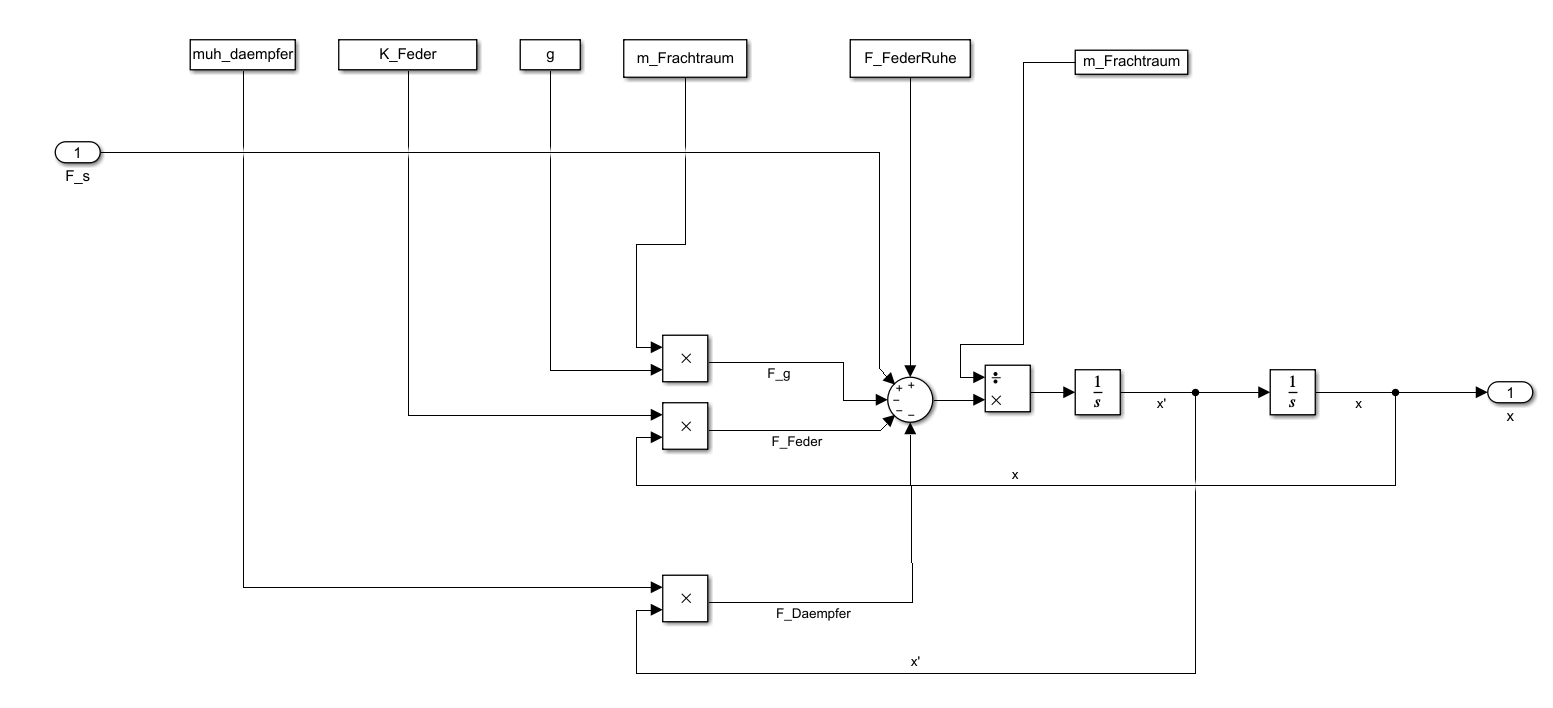
\includegraphics[width=0.7\textwidth]{Bilder/SimulinkStreckenModell.PNG}
		\caption{Simulink Modell der Regelstrecke}
		\label{SimulinkStreckenModell}
	  \end{figure}
	
	\subsection{Formulierung der Frage}
	
	In this step, a question is derived from an observation or curiosity. It is a question which usually asks for an explanation such as ``Which control strategy is the best to control the position of an elevator?'' The question and the background of this question is usually formulated in the \emph{Introduction} and/or ``Project targets''.
	
	\subsection{Hyphothese}
	
	A hypothesis is a conjecture to which you arrive by following logical and theoretical steps. The necessary theory involved in your questioning is written in the section \emph{Theory}.
	
	\subsection{Prediction}
	
	In this step you define the possible outcomes of your hypothesis and show how do you arrive to them. In engineering this would be the design process and is usually presented in the section regarding \emph{Methodology}.
	
	\subsection{Testing}
	
	Your hypothesis/design must be critically analysed and validated. For this you need to test it (by means e.g. of simulation). Your findings come in the section \emph{validation}.
	
	\subsection{Analysis}
	
	Through analysis of the results you may conclude if your hypothesis was correct or not. You should also explain what went wrong, under which circumstances the hypothesis would be right, etc. These findings come into the section \emph{Conclusions}.
	
	\section{Methodology} 
	
	In order to have a fast and homogeneous evaluation you should follow the rules laid out in the next subsections.
	
	\subsection{Structure}
	
	All reports must have the same structure at the \emph{section} level. Subsections may be adapted according to the specifics of the project. Table~\ref{tbl:sections} shows the required names in English and German.
	
	\begin{table}[hb]
		\caption{Required section headers in the project}\label{tbl:sections}
		\centering
		\begin{tabular}{cp{12em}p{12em}}
			\hline
			\bfseries Nr. & \bfseries English & \bfseries German\\
			\hline
			I & Introduction & Einführung\\
			II & Project targets & Projektziele \\
			III & Theory & Theorie \\
			IV & Methodology (Controller design) & Methodik (Reglerentwurf)\\
			V & Validation (Parameter tuning) & Validierung/Test \\
			VI & Observations and other effects & Beobachtungen und andere Effekte\\
			VII & Conclusions & Schlussfolgerungen\\
			\hline
		\end{tabular}
	\end{table}
	

	\subsection{Length}
	
	There is no minimum length, however, the report must include a comprehensible explanation of the different sections. The maximum length for the report is 8 pages.


	
	\subsection{Design}
	
	\subsubsection{General design}
	
	Tue work must be presented as a two column article with a serif font (Computer modern, Times, etc.)  size of minimum 9\,pt and a maximum of 10\,pt. The margins should be within 1\,cm and 2\,cm.
	
	\subsubsection{Figures and Tables}
	Tables and figures must be captioned (Tables above, Figures below) and \emph{must be referenced in the document}. Both tables and figures may be presented in one column or in both columns as depicted in Figure~\ref{fig:doublecolumn}. Please do not include two-column tables or figures in the first page!
	

	
	\subsubsection{Formulae}
	Formulae shall be enumerated and can be referenced such as (\ref{eq:einstein}) if necessary.
	
	\begin{equation}
		E=m\cdot c^2 \label{eq:einstein}
	\end{equation}
	
	\subsubsection{References}
	References must be clearly and unequivocal stated and must be quoted. Inline quoting can be ``Important debates in the history of science concern rationalism''\cite{scientificMethod}. Block quoting can be:
	\begin{quotation}
		Important debates in the history of science concern rationalism, especially as advocated by René Descartes; inductivism and/or empiricism, as argued for by Francis Bacon, and rising to particular prominence with Isaac Newton and his followers; and hypothetico-deductivism, which came to the fore in the early 19th century.\cite{scientificMethod}
	\end{quotation}
	
	References may be used either via BibTeX of they could be written in the document as presented in this example. In any case, the references must include author, title, edition and pages for printed media or URL and last access for electronic media. Please remember that an electronic book is still a printed media.
	
	\section{Validation}
	
	The project report and presentation will account for 100\% of your grade. The marking scheme is based on a 100-point scale and is distributed through the criteria presented in Table~\ref{tbl:grading}.
	
	\begin{table*}[h]
		\caption{Grading scheme for projects in SoSe 2020}\label{tbl:grading}
		\centering
		\begin{tabular}{l p{0.13\linewidth} p{0.5\linewidth} c}
			\hline
			\bfseries \# & \bfseries Evaluation point & \bfseries Criteria & \bfseries Points \\
			\hline
			1 & Introduction (10) & Is present & 1 \\
			\cline{3-4}
			 & & Clearly states the problem & 6 \\
			 \cline{3-4}
			 & & Clearly states the relevance of the problem & 3\\
			 \hline
			 2 & Project targets (10) & Is present & 1 \\
			 \cline{3-4}
			 & & Problem is correctly defined & 6 \\
			\cline{3-4}
			 & & Expected outcomes are clearly stated & 3 \\
			 \hline
			 3 & Theory & Is present & 1 \\
			\cline{3-4}
			 & & The proposed model covers the important/relevant characteristics & 6 \\
			\cline{3-4}
			 & & The model is so described that it can be reproduced & 3\\
			 \hline
			 4 & Methodology & Is present & 1 \\
			\cline{3-4}
			 & & Method is clearly stated (e.g. which controller will be used and why) & 6 \\
			\cline{3-4}
			 & & Preliminary results (as input for simulation/validation) are clearly stated & 3\\
			 \hline
			 5 & Validation & Is present & 1 \\
			\cline{3-4}
			  & & Results are plausible & 3\\
			\cline{3-4}
			  & & Results are discussed and potential limitations of the model are explained & 6\\
			 \hline
			 6 & Observations & Is present & 1\\
			\cline{3-4}
			& & Relevant effects are discussed & 3\\
			\cline{3-4}
			& & Explanations to the observed effects are relevant & 6\\
			\hline
			7 & Conclusions & Is present & 1 \\
			\cline{3-4}
			& & Conclusions address hypothesis and project aims and goals & 9 \\
			\hline
			8 & Final presentation & Sticks to 5 Minute maximum & 5 \\
			\cline{3-4}
			&& Presents the content professionally & 5\\
			\cline{3-4}
			&& Addresses all sections of the report & 10 \\
			\cline{3-4}
			&& Public can understand about the project, solution and effects even if they have little experience on the specific topic & 10\\
			\hline
			\hline
			 & Total & & 100 \\
		\end{tabular}
	\end{table*}

	\subsection{Points grading scheme}
	
	In all categories, there is the possibility of having either one, three, six or nine points. One-point rubrics are graded on present/not present. If the section is not present, the student will lose the point.
	
	Three-, six- and nine-point rubrics are graded as follows:
	
	\begin{enumerate}
		\item One third of the points are awarded if the grading rubric represents the minimum effort necessary to comply with it (read and quote).
		\item Two thirds of the points are awarded if the student is able to explain the required information  (interpret and apply).
		\item The full points are awarded if the student is able to interpret the information, apply it and discuss it.
	\end{enumerate}

	{\bfseries Example:} Describe the transfer function of an RC filter (input to output voltage) for 6 points
	
	\begin{description}
		\item[0p] $U_{C} = \frac{1}{C}\int i_{c} \cdot dt$
		\item[2p] Prof. Notholt says in script: $G(s) = \frac{1}{RCs+1}$
		\item[4p] ``The transfer function is the quotient of the Laplace input signal to the Laplace output signal'' [Lunze 1999] thus being $G(s) = \frac{1}{Ts+1}$ with $T=RC$
		\item[6p] The RC filter can be considered like a complex voltage divider with $Z = 1/sC$, the solution is then $U_{C} = \frac{1/sC}{R + 1/sC} \cdot U_\textrm{e}$ or, simplified and as transfer function: $G(s) = U_{C}/U_\textrm{e} = \frac{1}{RCs + 1}$ 
	\end{description}
	
	
	\section{Conclusions}
	
	This paper has described the minimum requirements for the written project and final presentation. Please meake sure you read this document completely and follow the guidelines. Prof. Notholt wish you the best for your endeavor!


	
	\begin{thebibliography}{1em}
		\bibitem{scientificMethod} Wikipedia, ``The scientific method'', online, \url{https://en.wikipedia.org/wiki/		 
		Scientific_method}, accessed 20.4.2020.
	\end{thebibliography}

\end{document}